\chapter{The pseudoinverse}
\label{chap:pseudoinverse}
The pseudoinverse, or generalized matrix inverse, is a powerful tool in the study of linear systems. We have seen already how this generalization is a potent tool in the arena of least squares problems. We will go on to see that the pseudoinverse and the \svdl \ work together like hand and glove.

%%
\section{Definition of the matrix pseudoinverse}
Can the matrix inverse be generalized? Can we find a consistent framework to talk about the inverse of a rectangular matrix? A singular matrix? Why would we search for such a beast?

We have seen in chapter \eqref{chap:simple} that general linear systems do not have an inverse, but they still offer a least squares solution. A reasonable expectation would be to connect the least squares solution with a generalized matrix inverse. In fact we saw that a generalized inverse would allow a direct solution to the least squares problem. 

The generalized matrix inverse also offers generalized nomenclature. It is also known as the pseudoinverse or the Moore-Penrose inverse.

Connect to the Drazin inverse.

So the concept of a generalized inverse is not far fetched. However, important theoretical work needed to be done to solidify the ideas. We begin with important guidelines which serve 
An elegant collection of necessary and conditions define the pseudoinverse. These conditions are credited to Sir Arthur Penrose, \cite[Penrose].

\begin{thm}
The matrix $\G{}$ is a pseudoinverse of the matrix $\A{}$ if and only these four properties are satisfied:
\begin{enumerate}
\item $\A{}\G{}\A{} = \A{}$
\item $\G{}\A{}\G{} = \G{}$
\item $\paren{\A{}\G{}}^{*} = \A{}\G{}$
\item $\paren{\G{}\A{}}^{*} = \G{}\A{}$
\end{enumerate}
%\label{thm:Penrose}
\end{thm}

Notice the conventional inverse also satisfies these four properties.
%
\subsection{Verifying the pseudoinverse}
The key to checking the Penrose conditions in %\eqref{thm:Penrose}
is to compute the products $\aap{*}$ and $\apa{*}$. If they are Hermitian, then the last two conditions are satisfied. We will see shortly that these matrix products play important roles as projectors.

\subsubsection{First example matrix}
The first example has
\begin{equation}
  \A{} = \Aexample, \qquad \Ap = \Aexamplepi.
\end{equation}
The matrix products are then
\begin{equation}
  \leftinv = \AexampleApA, \qquad \rightinv = \AexampleAAp,
  \label{eq:mp:projectors:1}
\end{equation}
both of which are clearly symmetric and therefore the last two Penrose conditions are met. The first two Penrose tests are these:
\begin{equation}
  \begin{split}
     \mpcone &= \Aexample\AexampleApA = \Aexample = \A{};
  \end{split}
\end{equation}
\begin{equation}
  \begin{split}
     \mpctwo &= \AexampleApA\Aexamplepi = \Aexamplepi = \Ap.
  \end{split}
\end{equation}
%

\subsubsection{Second example matrix}
The second example matrix has these definitions:
\begin{equation}
  \A{} = \matrixbravo, \qquad \Ap = \matrixbravopi.
\end{equation}
Because this matrix has full row rank the pseudoinverse is a right inverse:
\begin{equation}
  \leftinv = \matrixbravoApA, \qquad \rightinv = \matrixbravoAAp = \I{2}.
  \label{eq:mp:projectors:2}
\end{equation}
As before, both of these are symmetric and therefore the last two Penrose conditions are met. Because this matrix has full row rank, the pseudoinverse is also a right-inverse. The first two Penrose tests are these:
\begin{equation}
  \begin{split}
     \mpcone &= \I{2}\A{} = \A{};
  \end{split}
\end{equation}
\begin{equation}
  \begin{split}
     \mpctwo &= \Ap\I{2} = \Ap.
  \end{split}
\end{equation}

\subsubsection{Third example matrix}
The third and final example matrix has these definitions:
\begin{equation}
  \A{} = \matrixbravo, \qquad \Ap = \itwo.
\end{equation}
Because this matrix is square and has full rank, it possesses a standard inverse:
\begin{equation}
  \leftinv = \rightinv = \A{}.
  \label{eq:mp:projectors:2}
\end{equation}
As before, both of these are symmetric and therefore the last two Penrose conditions are met. Because this matrix has full row rank, the pseudoinverse is also a right-inverse. The first two Penrose tests are these:
\begin{equation}
  \begin{split}
     \mpcone &= \I{2}\A{} = \A{};
  \end{split}
\end{equation}
\begin{equation}
  \begin{split}
     \mpctwo &= \Ap\I{2} = \Ap.
  \end{split}
\end{equation}

%
%%%%%%%%%%%%%%%%%%%%%%%%%%%%%
\section{$\sig{}$ gymnastics}
Mastering manipulations of the SVD requires a thorough understanding of the basics of the $\sig{}$ matrix. The ideas are simple, yet experience shows this is the area where many mistakes are made.

The critical insight is that the $\sig{}$ matrix is the matrix of singular values $\ess{}$ held in a sabot matrix with zeros. This is apparent in block form:
\begin{equation}
  \sig{} = \essmatrix{}
\end{equation}
where the block matrix $\zero$ represents a matrix of zeros of the required dimension. While this notation helps clarify what these matrices are being multiplied together, it has a drawback: the matrices $\sig{}$ and $\sig{T}$ have the same block structure. There are two reasons for this:
\begin{enumerate}
\item the $\ess{}$ matrix is diagonal, hence $\ess{}=\ess{T}$;
\item the $\zero$ applies to any size matrix of zeros.
\end{enumerate}
\begin{equation}
  \begin{split}
     \sig{} &= \essmatrix{},\\
     \sig{T}&= \essmatrix{T} = \essmatrix{}.
  \end{split}
\end{equation}

One fix is to specify the dimensions in the matrix statement like so:
\begin{equation}
  \begin{split}
     \sig{} &= \essmatrix{}^{\by{m}{n}},\\
     \sig{T}&= \essmatrix{}^{\by{n}{m}}.
  \end{split}
\end{equation}
This can be unwieldily. In general we will avoid the bulkier notation and rely upon the reader being able to read the implied dimensions in the problem statement. To that end, some practice is needed.

Perhaps the most confusing details involve the sabot matrix $\sig{}$. This container of zeros has the same shape as the target matrix. It contains a diagonal matrix $\textbf{S}$ of non-zero singular values.

Because the matrix of singular values is square we have the following two identities:
\begin{equation*}
  \ess{} = \ess{T} = \Smatrix, \qquad \ess{-1} = \Smatrixinv,
\end{equation*}
\begin{equation*}
  \ess{}\,\ess{T} = \ess{T}\ess{} = \ess{2}.
\end{equation*}

\begin{table}[htdp]
\begin{center}
\begin{tabular}{lclccc}
  form && block matrix &&& dimension \\\hline
  $\sig{}$   &=& $\mat{cc}{\ess{} & \zero \\ \zero & \zero}$  &&& $m \times n$ \\
  $\sig{T}$  &=& $\mat{cc}{\ess{T} & \zero \\ \zero & \zero}=\mat{cc}{\ess{} & \zero \\ \zero & \zero}$  &&& $n \times m$ \\
  $\sig{(+)}$&=& $\mat{cc}{\ess{-1} & \zero \\ \zero & \zero}$ &&& $n \times m$ \\
%%%
  $\sig{}\sig{T}$  &=& $\mat{cc}{\ess{} & \zero \\ \zero & \zero}\mat{cc}{\ess{T} & \zero \\ \zero & \zero}$ &=& $\mat{cc}{\ess{2} & \zero \\ \zero & \zero}$ & $m \times m$ \\
  $\sig{T}\sig{}$  &=& $\mat{cc}{\ess{T} & \zero \\ \zero & \zero}\mat{cc}{\ess{} & \zero \\ \zero & \zero}$ &=& $\mat{cc}{\ess{2} & \zero \\ \zero & \zero}$ & $n \times n$ \\
  $\sig{}\sig{(+)}$&=& $\mat{cc}{\ess{} & \zero \\ \zero & \zero}\mat{cc}{\ess{-1} & \zero \\ \zero & \zero}$ &=& $\mat{cc}{\I{\rho} & \zero \\ \zero & \zero}$ & $m \times m$ \\
  $\sig{(+)}\sig{}$&=& $\mat{cc}{\ess{-1} & \zero \\ \zero & \zero}\mat{cc}{\ess{} & \zero \\ \zero & \zero}$ &=& $\mat{cc}{\I{\rho} & \zero \\ \zero & \zero}$ & $n \times n$ \\[15pt]
%%%
  $\sig{(+)}\sig{}\sig{T}$&=& $\mat{cc}{\I{\rho} & \zero \\ \zero & \zero}\mat{cc}{\ess{} & \zero \\ \zero & \zero}$ &=& $\sig{}$ & $m \times n$ \\[15pt]
  $\sig{T}\sig{}\sig{(+)}$&=& $\mat{cc}{\ess{T} & \zero \\ \zero & \zero}\mat{cc}{\I{\rho} & \zero \\ \zero & \zero}$ &=& $\sig{T}$ & $n \times m$ \\[15pt]
\end{tabular}
\end{center}
\label{default}
\caption[$\sig{}$ and $\sig{T}$ have the same block structure]{Note that although the matrices $\sig{}$ and $\sig{T}$ have the same block structure (because $\ess{}=\ess{T}$), the matrix and its transpose have different dimensions.}
\end{table}%

\begin{table}[htdp]
\begin{center}
\begin{tabular}{ll|ccc}
  form & block matrix & example 1 & example 2 & example 3  \\\hline
  $\sig{}$  & $\mat{cc}{\ess{} & \zero \\ \zero & \zero}$  & $\Sigmaexampleb$ & $\matrixbravosigma$ & $\matrixalphasigma$ \\
  $\sig{T}$ & $\mat{cc}{\ess{T} & \zero \\ \zero & \zero}$ & $\Sigmatexample$ & $\matrixbravosigmat$ & $\matrixalphasigmat$ \\
  $\sig{(+)}$& $\mat{cc}{\ess{-1} & \zero \\ \zero & \zero}$  & $\Sigmaexamplepi$ & $\matrixbravosigmapi$ & $\matrixalphasigmapi$ \\
%%%
  $\sig{}\sig{T}$ & $\mat{cc}{\ess{2} & \zero \\ \zero & \zero}$ & $\mat{c|cc}{6&0&0\\\hline0&0&0\\0&0&0}$ & $\mat{cc}{15 & 0 \\0&3}$ & $\mat{cc}{8&0\\0&2}$\\
  %%%
  $\sig{T}\sig{}$ & $\mat{cc}{\ess{2} & \zero \\ \zero & \zero}$ & $\mat{c|c}{6&0\\\hline0&0}$ & $\mat{cc|c}{15&0&0 \\0&3&0\\\hline0&0&0}$ & $\mat{cc}{8&0\\0&2}$ \\
  %%%
  $\sig{}\sig{(+)}$& $\mat{cc}{\I{\rho} & \zero \\ \zero & \zero}$ & $\mat{c|cc}{1&0&0\\\hline0&0&0\\0&0&0}$ & $\itwo$ & $\itwo$ \\
  $\sig{(+)}\sig{}$& $\mat{cc}{\I{\rho} & \zero \\ \zero & \zero}$ & $\mat{c|c}{1&0\\\hline0&0}$ & $\mat{cc|c}{1&0&0\\0&1&0\\\hline0&0&0}$ & $\itwo$ \\[15pt]
\end{tabular}
\end{center}
\label{default}
\caption[$\sig{}$ gymnastics for our well-worn example matrices]{$\sig{}$ gymnastics for our well-worn example matrices. Note that although the matrices $\sig{}$ and $\sig{T}$ have the same block structure (because $\ess{}=\ess{T}$), the matrix and its transpose have different dimensions.}
\end{table}%

 As an example a matrix $\A{}\in\cmplx{\by{4}{3}}_{2}$ the sabot matrix looks like
\begin{equation}
  \sig{} = \essmatrix{} = 
  \mat{cc|c}{\sigma_{1}&0&0\\0&\sigma_{2}&0\\\hline0&0&0\\0&0&0}.
\end{equation}
The transpose behaves as expected:
\begin{equation}
  \sig{T} = \essmatrix{T} = 
  \mat{cc|cc}{\sigma_{1}&0&0&0\\0&\sigma_{2}&0&0\\\hline0&0&0&0}.
\end{equation}

The confusion comes when we try to invert the sabot matrix. The singular value matrix $\textbf{S}$ inverts easily: just take the reciprocal of the diagonal entries. But what about the sabot entries? By looking at the conformability we see that we must also take the transpose of the sabot matrix. That is, if we want to multiply the size $\by{m}{n}$ sabot by its inverse on either the right or the left the inverse must have size $\by{n}{m}$. To form the inverse of the sabot matrix $\sig{}$ form the transpose and invert the matrix $\textbf{S}$. To remind us that this is special process use the following symbol
\begin{equation}
  \sig{(+)} = \mat{c|c}{\textbf{S}^{-1} & \zero \\\hline \zero & \zero} = 
  \mat{cc|cc}{\frac{1}{\sigma_{1}}&0&0&0\\0&\frac{1}{\sigma_{2}}&0&0\\[3pt]\hline0&0&0&0}.
\end{equation}

%%
\section{Practice}
We should practice the $\sig{}$ gymnastics as they are at the heart of using the SVD in matrix analysis. 

%%%
\subsection{Transpose relations}
A good place to start is with the product matrices
\begin{equation}
  \begin{split}
    \prdmy{*} = \paren{ \svd{*} } \paren{ \svdt{*} } = \wx{*},\\
    \prdmx{*} = \paren{ \svdt{*} }\paren{ \svd{*} }  = \wy{*}.\\
  \end{split}
\end{equation}
These are the crucial matrices needed to find the \svdl \ and they involve the matrix products $\sx$ and $\sy$. Though these matrices have the same block structure, they have different dimensions.
\begin{equation}
  \begin{split}
  \sig{T}\sig{} &= 
  \essmatrix{T}^{\by{n}{m}}_{\rho} 
  \essmatrix{}^{\by{m}{n}}_{\rho} = 
  \essmatrix{2}^{\by{n}{n}}_{\rho} \\
  \sig{}\,\sig{T} &= 
  \essmatrix{}^{\by{m}{n}}_{\rho} 
  \essmatrix{T}^{\by{n}{m}}_{\rho} = 
  \essmatrix{2}^{\by{m}{m}}_{\rho}
  \end{split}
\end{equation}
These are the special cases where there is no sabot:
\begin{enumerate}
\item if $\rho=m$ then $\sy = \ess{2}$;
\item if $\rho=n$ then $\sx = \ess{2}$;
\item if $\rho=m=n$ then $\sx = \sy = \ess{2}$.
\end{enumerate}

%%%
\subsection{Inverse relations}
No consider the product matrices
\begin{equation}
  \begin{split}
    \invy{*} = \paren{ \svd{*} } \paren{ \mpgi{*} } = \vx{*},\\
    \invx{*} = \paren{ \mpgi{*} }\paren{ \svd{*} }  = \vy{*}.\\
  \end{split}
\end{equation}
These matrices are used to define the fundamental projectors. Again we have the same block structure despite having different dimensions.
\begin{equation}
  \begin{split}
  \sig{\pssymbol}\sig{} &= 
  \essmatrix{-1}^{\by{n}{m}}_{\rho} 
  \essmatrix{}^{\by{m}{n}}_{\rho} = 
  \idmatrix{\rho}^{\by{n}{n}}_{\rho} = \J{n}{\rho} \\
  \sig{}\,\sig{\pssymbol} &= 
  \essmatrix{}^{\by{m}{n}}_{\rho} 
  \essmatrix{-1}^{\by{n}{m}}_{\rho} = 
  \idmatrix{\rho}^{\by{m}{m}}_{\rho} = \J{m}{\rho}
  \end{split}
\end{equation}
Because we encounter these matrices regularly, they have their own name and symbol. They are truncated identity matrices, $\J{}{}$. We will see them play a central role in the theory of fundamental projectors. But first, a quick example:
For example, for $\A{}\in\cmplx{\by{3}{4}}_{2}$
\begin{equation}
  \begin{split}
  \sig{(+)}\sig{} &= 
  \mat{cc|cc}{1&0&0&0\\0&1&0&0\\\hline0&0&0&0\\0&0&0&0} = \J{4}{2} \\
  \sig{}\,\sig{(+)} &= 
  \mat{cc|c}{1&0&0\\0&1&0\\\hline0&0&0} = \J{3}{2}
  \end{split}
\end{equation}
The $\J{}{}$ matrices act as stencils, letting only parts of matrices interact on multiplication. This diagram shows how a stencil blocks the shaded part of the matrices from multiplying. For the SVD, the unshaded columns represent the range space vectors and the shaded columns the null space vectors.
%%
\subsection{Truncated identity}
\begin{figure}[htbp] %  figure placement: here, top, bottom, or page
   \centering
   \includegraphics[ ]{pdf/svd/mask_06_04_04} 
   \caption[The stencil action of the truncated identity matrix]{The stencil action of the truncated identity matrix. On the left we see vectors shaded. These vectors not contribute to the product because of the stencil action. . The matrix product is equivalent to the one on the right which uses matrices with the appropriate rows and columns deleted.}
   \label{fig:svd:stencil}
\end{figure}
Here is a product that is common when working with the SVD. Notice how the stencil ``knocks out'' the null space components:
\begin{equation}
  \begin{split}
    \invx & = \wx{*} \\
    &= \xrn{} \J{n}{\rho} \xtrn{*} \\
    &= \xrng{} \xrng{*}.
  \end{split}
\end{equation}


%%
\subsection[Construction: general case]{Constructing the pseudoinverse when $\A{}$ is singular}
Let's back up and look at the process more carefully.
Given a \svdl \ decomposition, how do we construct the pseudoinverse? The simplest step would be to apply the inverse operation to the decomposition. The domain matrices invert easily - they are orthogonal, so forming the Hermitian conjugate forms the inverse. The sticky issue comes from the matrix of singular values, $\sig{}$. How should we ``invert'' a matrix which is not square and which may have zero elements on the lower diagonals?

If two matrices $\U{}$ and $\V{}$ are both nonsingular, then we can relate the inverse of the product to the product of the inverses:
\begin{equation}
  \paren{\U{}\V{}}^{-1} = \V{-1}\U{-1}.
\end{equation}

Consider the case of a nonsingular matrix $\A{}$.
\begin{equation}
  \paren{\A{}}^{-1} \Rightarrow \paren{\svd{*}}^{-1} \Rightarrow \paren{\X{*}}^{-1}\paren{\sig{}}^{-1}\paren{\Y{}}^{-1}=\X{}\,\sig{-1}\,\Y{*}.
\end{equation}
Because the domain matrices are unitary, their inverses are trivial to compute: form the Hermitian conjugate. When the target matrix is nonsingular the $\sig{}$ matrix is diagonal and can also be inverted easily.

Retreat to the safe case: when $\sig{}$ is square and diagonal with a full diagonal with no zero elements. There we would invert the diagonal elements like so
\begin{equation}
  \begin{split}
   \sig{}       & \quad \Rightarrow \quad \sig{-1},\\    
   \sig{}_{k,k} & \quad \Rightarrow \quad \frac{1}{\sig{}_{k,k}}, \quad k=1,2,\dots,\rho.    
  \end{split}
\end{equation}This motivates us to move to the pathological cases and simply invert all of the singular values. By definition, in this work singular values are non-zero. In order to be conformable we also need to form the transpose.

To invert a singular \index{singular values matrix!inversion}singular values matrix $\sig{}$, perform these two steps:
\begin{enumerate}
\item form the transpose matrix $\sig{T}$,
\item invert the singular values.
\end{enumerate}
In terms of the $\ess{}$ matrix the operations look like this:
\begin{equation}
  \begin{split}
    \sig{} &= \mat{c|c}
    {
    \ess{} & \zero \\\hline
    \zero & \zero
    }^{\paren{m\times n}} \\
    \sig{(+)} &= \mat{c|c}
    {
    \ess{-1} & \zero \\\hline
    \zero & \zero
    }^{\paren{n\times m}}
  \end{split}
\end{equation}
The trouble with this formulation is that it obscures the transpose of the sabot matrix.  Hopefully the examples will clarify this transposition of the sabot.

For our well-travelled example matrix this process looks like
\begin{equation}
\begin{array}{ccc}
\sig{} &\Rightarrow& \sig{(+)} \\
 \mat{c|c}{\sigma_{1} & 0\\\hline0 & 0 \\0 & 0} & \Rightarrow & \mat{c|cc}{\frac{1}{\sigma_{1}} & 0 & 0\\[3pt]\hline0 & 0 & 0} \\
\Sigmaexampleb  & \Rightarrow & \mat{c|cc}{\ssix & 0 & 0\\[4pt]\hline0 & 0 & 0}.
\end{array}
\end{equation}
Because the process is unique to the $\sig{}$ matrix, it uses a dedicated superscript ``(+)''. In conversational mathematics, we would say
\begin{quote}
  To form the inverse of the $\sig{}$ matrix of singular values invert all non-zero entries and form the transpose matrix.
\end{quote}

These simplistic, intuitive steps work. 
\begin{equation}
    \mpgiax{*}
\end{equation}
The relationships between \svdl s for the target matrix, the Hermitian conjugate and the psuedoinverse are shown here:
\begin{equation}
  \begin{array}{lcccc}
    \A{} &=& \Y{} & \sig{} & \X{*} \\
    \A{*} &=& \X{} & \sig{T} & \Y{*} \\
    \Ap &=& \X{} & \sig{(+)} & \Y{*} \\
  \end{array}
\end{equation}

%%
\subsection[Construction: special case]{Constructing the pseudoinverse when $\A{}$ is nonsingular}
For the case when the target matrix $\A{}$ is nonsingular there is no sabot matrix: $\sig{}=\ess{}$ and the inversion is process is
\begin{equation}
  \begin{split}
    \sig{} &= \ess{} \\
    \sig{(+)} &= \ess{-1}
  \end{split}
\end{equation}
Restated another way, a matrix is nonsingular if and only if the matrix of singular values fils the sabot matrix.
\begin{equation}
  \A{} \text{ is nonsingular}\qquad \iff \qquad \sig{}=\ess{}
\end{equation}
In these cases the $\sig{}$ matrix will be square and diagonal with no zero entries on the diagonal.

%%
\subsection[Verification: singular case]{Verification of the pseudoinverse: nonsingular case}

\endinput
\section{Chiral inverses}
\label{sec:chiral}
Chiral matrix inverses are inverses which operate on the left- or right-hand side of the target matrix. In analogy with the concept of chirality in chemistry, the chiral inverses have different shapes; in fact they are transposes.

%%
\subsection{Definitions}
For a target matrix $\A{}\in\cmplx{\by{m}{n}}_{\rho}$ the pseudoinverse $\Ap\in\cmplx{\by{n}{m}}_{\rho}$. That is the pseudoinverse has the shape of the transpose of the target matrix and retains the same rank. Figure \eqref{fig:mpp:chiral} shows when the pseudoinverse will be a chiral inverse. When the target matrix has full row rank ($\rho=m$), the pseudoinverse $\Ap$ is a right inverse. When the matrix has full column rank $\Ap$ is a left inverse. When the target matrix has full row and column rank it is square and the pseudoinverse is the standard inverse: $\Ap=\A{-1}$.

\begin{table}[htdp]
\begin{center}
\begin{tabular}{l|clc}
chirality, $\chi$ & requirement & equivalence & expression\\\hline
right & $\rho = m$ & $\Ap=\AinvR$ & $\rightinv=\I{m}$\\
left  & $\rho = n$ & $\Ap=\AinvL$ & $\leftinv=\I{n}$\\
ambichiral & $\rho=m=n$ & $\Ap=\A{-1}$ & $\rightinv=\leftinv=\I{m}$\\
ampichiral & $\rho< m,\rho< n$ & \quad none & $\rightinv\ne\I{m},\ \leftinv\ne\I{n}$\\
\end{tabular}
\end{center}
\label{fig:mpp:chiral}
\caption[Conditions for when the pseudoinverse is a chiral inverse]{Conditions for when the pseudoinverse is a chiral inverse. The conditions are when the target matrix has either full row rank or full column rank.}
\end{table}%

Examine cases illustrating the four different classifications for the actions of the pseudoinverse. The rules are basic:
\begin{enumerate}
\item If the matrix has full \textit{row} rank, the pseudoinverse is a \textit{right} inverse.
\begin{equation}
  \rho = m: \quad \Ap = \AinvL
\end{equation}
\item If the matrix has full \textit{column} rank, the pseudoinverse is a \textit{left} inverse.
\begin{equation}
  \rho = n: \quad \Ap = \AinvR
\end{equation}
\end{enumerate}

From this we conclude that if the matrix has full row rank and full column rank the pseudoinverse both a left and right inverse. That is, the pseudoinverse in the classic inverse.

We also conclude that if the matrix is rank deficient in both row and column then the pseudoinverse in neither a right not a left inverse.

Examples of all four cases follow.

%%%
\subsection{Ambichiral or classic inverse: $\Ap = \A{-1}$}
What are the two rank conditions?
\begin{enumerate}
\item The matrix has full row rank: $\rho = m$.
\item The matrix has full column rank: $\rho = n$.
\end{enumerate}
Therefore the matrix has $\rho$ row and $\rho$ columns. Therefore it is square and of full rank. We don't know what the rank is or what the size is, but we can state
\begin{equation}
  \rho = m = n.
\end{equation}

Choose a target matrix $\Arrr{2}{2}{2}$.
\begin{equation*}
  \begin{array}{ccccc}
    \A{} &=& \Y{} & \sig{} & \X{T} \\
    \matrixalpha &=
    & \matrixalphaY 
    & \matrixalphasigma 
    & \matrixalphaXt.
  \end{array}
\end{equation*}
The pseudoinverse is given by
\begin{equation*}
  \begin{array}{ccccc}
    \Ap &=& \X{} & \sig{(+)} & \Y{T} \\
    \matrixalphapi &=
    & \matrixalphaX 
    & \matrixalphasigmapi
    & \matrixalphaYt.
  \end{array}
\end{equation*}
The matrix products produce the same result:
\begin{equation*}
  \begin{array}{cccc}
  \A{}&\Ap&=&\I{2},\\
  \matrixalpha &
  \matrixalphapi & = &
  \itwo;\\[25pt]
  \Ap&\A{}&=&\I{2},\\
  \matrixalphapi &
  \matrixalpha & = &
  \itwo.
  \end{array}
\end{equation*}

\subsection{Right inverse only: $\Ap=\AinvR$}
What are the two rank conditions?
\begin{enumerate}
\item The matrix has full row rank: $\rho = m$.
\item The matrix has partial column rank: $\rho < n$.
\end{enumerate}
Therefore the matrix has $\rho$ rows and $\rho$ columns. Therefore it is square and of full rank. We don't know what the rank is or what the size is, but we can state
\begin{equation}
  \begin{split}
     \rho = m,\\
     \rho < n.
  \end{split}
\end{equation}

Consider a target matrix $\Arrr{2}{3}{2}$.
\begin{equation*}
  \begin{array}{ccccc}
  \A{} &=& \Y{} & \sig{} & \X{T}\\
  \matrixbravo &=
  & \matrixbravoY  
  & \matrixbravosigma
  & \matrixbravoXt.
  \end{array}
\end{equation*}
The pseudoinverse is constructed in this fashion:
\begin{equation*}
  \begin{array}{ccccc}
    \Ap &=& \X{} & \sig{(+)} & \Y{T} \\
    \matrixbravopi &=
    & \matrixbravoX 
    & \matrixbravosigmapi
    & \matrixbravoYt.
  \end{array}
\end{equation*}
Postmultiplication by the pseudoinverse produces an identity matrix:
\begin{equation*}
  \begin{array}{cccc}
    \A{}&\Ap&=&\I{2},\\
   \matrixbravo &
   \matrixbravopi &=&
   \itwo.
  \end{array}
\end{equation*}
The complementary result is not as nice. Premultiplication by the pseudoinverse produces this result:
\begin{equation*}
  \begin{array}{cccc}
    \Ap&\A{}&\in&\real{\by{3}{3}}_{2},\\
   \matrixbravopi &
   \matrixbravo &=&
   \frac{1}{5}
   \mat{ccc}
   {
   1&0&2\\
   0&5&0\\
   2&0&4
   }.
  \end{array}
\end{equation*}

%%%
\subsection{Left inverse only: $\Ap = \AinvL$}
The two rank conditions are these:
\begin{enumerate}
\item The matrix has partial row rank: $\rho < m$.
\item The matrix has full column rank: $\rho = n$.
\end{enumerate}
These two statements are equivalent to these mathematical relationships:
\begin{equation}
  \begin{split}
     \rho &= n, \\
     \rho &< m
  \end{split}
\end{equation}

The target matrix for this example is $\A{}\in\cmplx{\by{3}{2}}_{2}$
\begin{equation*}
  \begin{array}{ccccc}
  \A{} & = & \Y{} & \sig{} & \X{T},\\
  \mat{rr}{1&2\\0&2i\\1&-2} &=&
  \left[
\begin{array}{rc>{\columncolor{ltgray}}r}
  \frac{1}{\sqrt{3}} & \frac{1}{\sqrt{2}} & -\frac{1}{\sqrt{6}} \\
  \frac{i}{\sqrt{3}} & 0 & \frac{2i}{\sqrt{6}} \\
 -\frac{1}{\sqrt{3}} & \frac{1}{\sqrt{2}} & \frac{1}{\sqrt{6}}
\end{array}
\right] &
\left[
\begin{array}{cc}
 2 \sqrt{3} & 0 \\
 0 & \sqrt{2} \\\hline
 0 & 0
\end{array}
\right] &
\left[
\begin{array}{cc}
 0 & 1 \\
 1 & 0
\end{array}
\right]
  \end{array}.
\end{equation*}
The pseudoinverse is constructed as so:
\begin{equation*}
  \begin{array}{ccccc}
  \Ap & = & \X{} & \index{Sigma matrix!inverse}\sig{(+)} & \Y{*},\\
  \frac{1}{6}\left[
\begin{array}{crr}
 3 & 0 & 3 \\
 1 & -i & -1
\end{array}
\right] &=&
  \left[
\begin{array}{cc}
 0 & 1 \\
 1 & 0
\end{array}
\right]&
\left[
\begin{array}{cc|c}
 \frac{1}{2 \sqrt{3}} & 0 & 0 \\
 0 & \frac{1}{\sqrt{2}} & 0
\end{array}
\right] &
\left[
\begin{array}{rcr}
  \frac{1}{\sqrt{3}} & \frac{i}{\sqrt{3}} & -\frac{1}{\sqrt{3}} \\
  \frac{1}{\sqrt{2}} & 0                  &  \frac{1}{\sqrt{2}} \\
  \rowcolor{ltgray}
 -\frac{1}{\sqrt{6}} & \frac{2i}{\sqrt{6}} & \frac{1}{\sqrt{6}}
\end{array}
\right].
\end{array}
\end{equation*}
Premultiplcation by the pseudoinverse produces an identity matrix:
\begin{equation*}
  \begin{array}{cccc}
  \Ap&\A{}&=&\I{2},\\
  \frac{1}{6}\left[
\begin{array}{crr}
 3 &  0 & 3 \\
 1 & -i & -1
\end{array}
\right] &
  \mat{rr}{1&2\\0&2\\1&-2} & = &
  \itwo.
  \end{array}
\end{equation*}
Postmultiplcation by the pseudoinverse does not produce an identity matrix:
\begin{equation*}
  \begin{array}{cccc}
  \A{}&\Ap&\in&\real{\by{3}{3}}_{2},\\
  \mat{rr}{1&2\\0&2i\\1&-2} &
  \frac{1}{6}\left[
\begin{array}{crr}
 3 &  0 & 3 \\
 1 & -i & -1
\end{array}
\right]
   & = &
  \frac{1}{6}
\left[
\begin{array}{crr}
 5 & -2 i & 1 \\
 2 i & 2 & -2 i \\
 1 & 2 i & 5
\end{array}
\right]
  \end{array}
\end{equation*}

%%%
\subsection{Ampichiral or generalized inverse: $\Ap\ne\AinvB$}
The two rank conditions are these:
\begin{enumerate}
\item The matrix has partial row rank: $\rho < m$.
\item The matrix has partial column rank: $\rho < n$.
\end{enumerate}

The target matrix $\A{}\in\real{\by{3}{2}}_{1}$ is studied in the first chapter and the \svdl \ is presented in equation \eqref{eq:simple:svd}; the pseudoinverse is given in equation \eqref{eq:simple:mppdecomp}. The multiplicative properties follow.

%%%
Multiplication on the left by the pseudoinverse does not produce an identity matrix:
\begin{equation*}
  \begin{array}{cccc}
  \Ap&\A{}&\in&\real{\by{2}{2}}_{1},\\
  \Aexamplepi &
  \Aexample 
   & = &
  \frac{1}{2}
  \mat{rrr}{1&-1&\\-1&1}
  \end{array}.
\end{equation*}

%
Multiplication on the right by the pseudoinverse does not produce an identity matrix:
\begin{equation*}
  \begin{array}{cccc}
  \A{}&\Ap&\in&\real{\by{3}{3}}_{1},\\
  \Aexample &
  \Aexamplepi
   & = &
  \frac{1}{3}
  \mat{rrr}{1&-1&1\\-1&1&-1\\1&-1&1}
  \end{array}.
\end{equation*}

%%
\section{The $\sig{}$ matrix}
The condition for the chirality of the pseudoinverse is encoded in the $\sig{}$ matrices. That is, we can classify the chirality of the inverse (left, right, both, neither) simply by inspecting the $\sig{}$ matrix. 

These conditions are summarized in table \eqref{tab:mpp:chiralsigma}.
%%%%
\begin{table}[htdp]
\begin{center}
%
\begin{tabular}{l|rclcrcl}
    $\chi$  & product  && & iff & condition \\\hline
    left  & $\leftinv$  &$=$& $\I{n}$ & $\iff$ & $\sig{(+)}\sig{}$ &=& $\I{n}$\\
    right & $\rightinv$ &$=$& $\I{m}$ & $\iff$ & $\sig{}\sig{(+)}$ &=& $\I{m}$\\
    both  & $\rightinv = \leftinv$ &$=$& $\I{m}=\I{n}$ & $\iff$ & $\sig{}\,\sig{(+)}=\sig{(+)}\sig{}$ &=& $\I{m}$\\
    neither  & $\rightinv $ &$\ne$& $\I{m}$ & $\iff$ & $\sig{}\,\sig{(+)}$ &$\ne$& $\I{m}$\\
             & $\leftinv $  &$\ne$& $\I{n}$ &        & $\sig{(+)}\,\sig{}$ &$\ne$& $\I{n}$\\[5pt]
\end{tabular}
%
\end{center}
\label{tab:mpp:chiralsigma}
\caption[Necessary and sufficient conditions to classify chirality]{The necessary and sufficient conditions to classify the chirality of the pseudoinverse can be expressed in terms of the $\sig{}$ matrix.}
\end{table}%

In this case with full row rank the pseudoinverse is also a \index{right inverse}right inverse. In this case with full column rank the pseudoinverse is also a \index{left inverse}left inverse. When the matrix has full rank (the column rank equals the row rank) the pseudoinverse reverts to being the standard inverse. Table \eqref{tab:pmii:rank} summarizes these points.
\begin{table}[bottom]
\begin{center}
\begin{tabular}{lll}
rank condition   & \ parameters \ & \ inverse condition\\\hline\hline
full row rank    & \ $\rho = m $  & \ $\Ap = \AinvR$ \\[3pt]
full column rank & \ $\rho = n $  & \ $\Ap = \AinvL$ \\[3pt]\hline
full row and column rank \ & \ $\rho = m = n $ \ & \ $\Ap = \AinvL = \AinvR$\\  row and column rank deficit \ & \ $\rho < m, \rho < n $ \ & \ $\Ap \ne \AinvB$ \\[6pt]
\end{tabular}
\end{center}
\label{tab:pmii:rank}
\caption[Classifications of the pseudoinverse]{Classifications of the pseudoinverse depend upon the rank condition of the target matrix. We see a concise definition of when the pseudoinverse is also the standard matrix inverse.}
\end{table}%
%%%

The formulaically minded may prefer this more formal mathematical presentation:
\begin{equation}
  \begin{array}{rclrcr}
    \leftinv &=& \I{n}, & \quad \A{}&\in&\cmplx{\by{m}{n}}_{n},\\
    \rightinv &=& \I{m}, & \quad \A{}&\in&\cmplx{\by{m}{n}}_{m},\\
    \leftinv = \rightinv &=& \I{m}, & \quad \A{}&\in&\cmplx{\by{m}{m}}_{m}.\\
  \end{array}
\end{equation}

%%
\subsection{Demonstrations of the four types of chiral inverses}

%%
\subsubsection{$\Ap=\A{-1}$}
What are the two rank conditions?
\begin{enumerate}
\item The matrix has full row rank.
\item The matrix has full column rank.
\end{enumerate}
Therefore the matrix has $\rho$ row and $\rho$ columns. Therefore it is square and of full rank. We don't know what the rank is or what the size is, but we can state
\begin{equation}
  \rho = m = n.
\end{equation}

%%
\subsubsection{$\Ap=\AinvL$}
\label{sec:lchiral}
The two rank conditions are these:
\begin{enumerate}
\item The matrix has partial row rank.
\item The matrix has full column rank.
\end{enumerate}
These two statements are equivalent to these mathematical relationships:
\begin{equation}
  \begin{split}
     \rho &= n, \\
     \rho &< m
  \end{split}
\end{equation}

%%
\subsubsection{$\Ap=\AinvR$}
This example flips the tank conditions.
\begin{enumerate}
\item The matrix has full row rank.
\item The matrix has partial column rank.
\end{enumerate}
These two statements are equivalent to these mathematical relationships:
\begin{equation}
  \begin{split}
     \rho &= m, \\
     \rho &< n
  \end{split}
\end{equation}


%%
\subsubsection{$\Ap\ne\AinvB$}
The final case is the least restrictive.
\begin{enumerate}
\item The matrix has partial row rank.
\item The matrix has partial column rank.
\end{enumerate}
These two statements are equivalent to these mathematical relationships:
\begin{equation}
  \begin{split}
     \rho &< m, \\
     \rho &< n
  \end{split}
\end{equation}
We can make no statement about the relationship between the number of rows, $m$ and the number of columns, $n$.

%%
\subsection{Proximity}
A quick note before closing. What about the first result in equation \eqref{eq:gen:lr}? How ``close'' is this matrix to the identity matrix?
\begin{equation}
\normt{\leftinv-\I{m}} = 
\normt{\frac{1}{5}
  \mat{ccc}
  {
 1 & 0 & 2 \\
 0 & 5 & 0 \\
 2 & 0 & 4
  }
  -
  \ithree} = 1.
\end{equation}
We will see this last result a few more times.

\endinput
\section[The fundamental projections]{The four fundamental orthogonal projections}
\label{sec:orthproj}

One of the bonuses we reap from the pseudoinverse is the four fundamental orthogonal projections. Each of these matrices projects onto a specific vector space. The spaces are these:
\begin{enumerate}
\item the range $\rng{\A{}}$,
\item the orthogonal complement to the range, $\rng{\A{}}^{\perp}$,
\item the null space $\nll{\A{}}$,
\item the orthogonal complement to the null space, $\nll{\A{}}^{\perp}$.
\end{enumerate}

We can make a simple yet powerful observation about the projectors.
Given the $\pee{}_{\mathcal{V}}$, the projector onto an $m-$dimensional subspace $\mathcal{V}$, the projector onto the orthogonal complement is
\begin{equation}
  \pee{}_{\mathcal{V}^{perp}} = \I{m}-\pee{}_{\mathcal{V}}.
\end{equation}

Below are these projectors for a matrix $\Accmn_{\rho}$ with pseudoinverse $\Ap$:
\begin{equation}
\boxed{
  \begin{array}{lcllcl}
    \projra& = &\rightinv & \quad \projrap& = &\I{m}-\rightinv\\
    \projnap& =& \leftinv & \quad \projna& = &\I{n}-\leftinv\\    
  \end{array}
  }
  \label{eq:fourprojpi}
\end{equation}

%%
\subsection{Projection onto the range of $\A{}$}
Let's explore the matrix product
\begin{equation}
  \begin{split}
    \projra &= \rightinv,\\
    &= \Y{}\,\sig{}\,\sig{(+)}\Y{*},\\
    & = \Y{}\,\J{m}{\rho}\,\Y{*}.
  \end{split}
\end{equation}
The truncated identity is acting like screen which only allows the first $\rho$ column vectors of $\Y{}$ into play. These are the vectors which span the image of the target matrix.

%%
\subsection{Projection onto the orthogonal complement of the range of $\A{}$}
Now subtract this projector from the identity:
\begin{equation}
  \begin{split}
    \projrap& = \I{m}-\projra,\\
      &= \I{m}-\rightinv,\\
      &= \I{m} - \Y{}\,\J{m}{\rho}\,\Y{*}.
  \end{split}
\end{equation}

%%
\subsection{Projection onto the null space of $\A{}$}
\begin{equation}
  \begin{split}
    \projna &= \leftinv,\\
    &= \X{}\,\sig{+}\,\sig{}\X{*},\\
    & = \X{}\,\J{n}{\rho}\,\X{*}.
  \end{split}
\end{equation}The truncated identity is acting like screen which only allows 
%%
\subsection{Projection onto the orthogonal complement of the null space of $\A{}$}
Let's explore the matrix product
\begin{equation}
  \begin{split}
    \projnap& = \I{n}-\projna,\\
      &= \I{n}-\leftinv,\\
      &= \I{n} - \X{}\,\J{n}{\rho}\,\X{*}.
  \end{split}
\end{equation}

Below are the same projectors shown in \eqref{eq:fourprojpi} for the same matrix $\Accmn_{\rho}$ with \svdl\ $\svd{*}$:
\begin{equation}
\boxed{
  \begin{array}{lcllcl}
    \projra&  = &\pra{*}  & \qquad  \projrap & = & \I{m}-\pra{*}\\[3pt]
    \projnap& = &\pnap{*} & \qquad  \projna  & = & \I{n}-\pnap{*}\\    
  \end{array}
  }
  \label{eq:fourprojsvd}
\end{equation}

%%%
%%%
\subsection{Primitive example}
Consider the following simple matrix:
\begin{equation}
  \A{}= \mat{cc}{1&0\\0&1\\0&0}.
\end{equation}
Using SVD by inspection we write
\begin{equation}
\begin{split}
  \svda{T},\\
  &= \I{3}\, \A{}\, \I{2},\\
  &= \mat{cc>{\columncolor{ltgray}}c}{1&0&0\\0&1&0\\0&0&1} \mat{cc}{1&0\\0&1\\\hline0&0} \itwo.
\end{split}
\end{equation}
The pseudoinverse is then
\begin{equation}
  \begin{split}
     \mpgia{T}, \\
     & = \itwo \mat{cc|c}{1&0&0\\0&1&0} \mat{ccc}{1&0&0\\0&1&0\\\rowcolor{ltgray}0&0&1},\\
     & = \mat{ccc}{1&0&0\\0&1&0}.
  \end{split}
\end{equation}

The fundamental spaces are revealed in the SVD and listed in table \eqref{tab:proj:ff}.
\begin{table}[htdp]
\begin{center}
\begin{tabular}{lll}
 subspace & \qquad \qquad span & source\\\hline
 $\rng{\A{}}$  & $\spn\lst{\mat{c}{1\\0\\0},\mat{c}{0\\1\\0}}$ \qquad & $\spn\lst{\Y{}_{*,1},\Y{}_{*,2}}$\\[19pt]\hline
 $\nll{\A{T}}$ & $\spn\lst{\mat{c}{0\\0\\1}}$ & $\spn\lst{\Y{}_{*,3}}$ \\[19pt]\hline
 $\rng{\A{T}}\qquad $ & $\spn\lst{\mat{c}{1\\0},\mat{c}{0\\1}}$ & $\spn\lst{\X{}_{*,1},\X{}_{*,2}}$\\[13pt]\hline
 $\nll{\A{}}$  & \qquad \qquad  $\emptyset$ & \quad  \quad $\emptyset$\\[2pt]\hline
\end{tabular}
\end{center}
\label{tab:proj:ff}
\caption{The fundamental spaces are revealed in the SVD. The codomain matrix $\Y{}$ encodes the vector spaces for the range of $\A{}$, $\rng{\A{}}$ and  the null space of the transpose, $\nll{\A{T}}$. The domain matrix $\X{}$ encodes the vector spaces for the range of the transpose $\A{T}$, $\rng{\A{T}}$ and  the null space of $\A{}$, $\nll{\A{}}$.}
\end{table}%

The analagous projectors are shown in table \eqref{tab:proj:fp}. The projection operators are these:
\begin{equation}
  \begin{array}{lcllcl}
    \projra& = &\rightinv = \mat{ccc}{1&0&0\\0&1&0\\0&0&0} & \quad \projrap& = &\I{m}-\projra = \mat{ccc}{0&0&0\\0&0&0\\0&0&1}\\
    \projnap& =& \leftinv = \itwo & \quad \projna& = &\I{n}-\projnap = \mat{cc}{0&0\\0&0}\\    
  \end{array}
  \label{eq:primitives}
\end{equation}
%%
\begin{table}[htdp]
\begin{center}
\begin{tabular}{llc}
 projection \\
 onto & \qquad vector space & projector\\\hline
 $\rng{\A{}}$  & $\spn\lst{\mat{c}{1\\0\\0},\mat{c}{0\\1\\0}}$ \qquad & $\mat{ccc}{1&0&0\\0&1&0\\0&0&0}$\\[19pt]\hline
 $\rng{\A{}}^{\perp}$ & $\spn\lst{\mat{c}{0\\0\\1}}$ & $\mat{ccc}{0&0&0\\0&0&0\\0&0&1}$ \\[19pt]\hline
 $\nll{\A{T}}\qquad $ & $\spn\lst{\mat{c}{1\\0},\mat{c}{0\\1}}$ & $\itwo$\\[13pt]\hline
 $\nll{\A{T}}^{\perp}$  & \qquad \qquad  $\emptyset$ & $\emptyset$\\[2pt]\hline
\end{tabular}
\end{center}
\label{tab:proj:fp}
\caption{The four fundamental projectors constructed from the target matrix $\A{}$ and the pseudoinverse $\A{T}$.}
\end{table}%

Study the action of the projectors on arbitrary vectors from the domain and the codomain. Because the target matrix is row rank deficient, there will be a null space as shown by the shaded column in the $\Y{}$ matrix. For the codomain the projection actions are these:
\begin{equation}
  \projra (y) = \mat{ccc}{1&0&0\\0&1&0\\0&0&0} 
     \mat{c}{y_{1}\\y_{2}\\y_{3}} = \mat{c}{y_{1}\\y_{2}\\0},
     \label{eq:mpp:red}
\end{equation}
\begin{equation}
  \projrap (y) = \mat{ccc}{0&0&0\\0&0&0\\0&0&1} 
     \mat{c}{y_{1}\\y_{2}\\y_{3}} = \mat{c}{0\\0\\y_{3}}.
     \label{eq:mpp:blue}
\end{equation}
The first case shows that the operator $\projra$ acts on vectors and projects them onto the $y_{1}-y_{2}$ plane. The complementary operator $\projra$ projects onto $y_{3}$ axis. These actions are shown graphically in figure \eqref{fig:projections3d}.

The case for the domain projection is trivial because the target matrix has full column rank.
\begin{equation}
  \projnap (x) = \itwo \mat{c}{x_{1}\\x_{2}} = \mat{c}{x_{1}\\x_{2}}.
\end{equation}

\begin{figure}[htbp] %  figure placement: here, top, bottom, or page
   \centering
   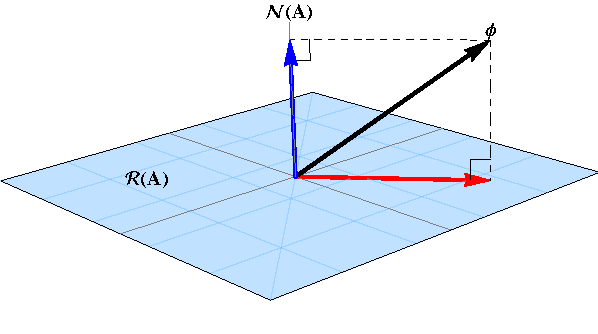
\includegraphics[]{pdf/mpp/projections} 
   \caption{Codomain projection examples. An arbitrary vector $\phi$ is represented by the black arrow. The red arrow shows the orthogonal projection onto the range of $\A{}$ as given by $\projra\paren{\phi}$ as shown in equation \eqref{eq:mpp:red}. The blue arrow shows the orthogonal projection onto the perpendicular complement of range of $\A{}$ as given by $\projrap\paren{\phi}$ as shown in equation \eqref{eq:mpp:blue}.}
   \label{fig:projections3d}
\end{figure}

%%
\subsection{Canonical example}
To solidify the theory work through one more example explicitly. This will show both formulations of the four fundamental projectors: using the pseudoinverse and using the component matrices from \svdl.

Start with the target matrix and the pseudoinverse:s 
\begin{equation}
  \A{} = \Aexample, \quad \Ap = \Aexamplepi.
\end{equation}

The projection onto the range of $\A{}$ is calculated in two different ways.
\begin{equation}
\begin{split}
  \projra &= \leftinv = \rthree
    \mat{rrr}
    { 
    1 & -1 &  1\\
   -1 &  1 & -1\\
    1 & -1 &  1\\
    }.
\end{split}
\end{equation}
However, we can bypass assembling the pseudoinverse and work directly with the decomposition matrices like so:
\begin{equation}
\begin{split}
  \projra &= \Y{}\,\sig{}\,\sig{(+)}\Y{T},\\
    & = \Y{}\,\J{m}{\rho}\,\Y{T},\\
    &= \Yshade \mat{ccc}{1&0&0\\0&0&0\\0&0&0} \Ytshade,\\
    &= \rthree
    \mat{rrr}
    { 
    1 & -1 &  1\\
   -1 &  1 & -1\\
    1 & -1 &  1\\
    }.
\end{split}
\end{equation}

The projection onto the perpendicular complement space  is this
\begin{equation}
  \projrap = \I{3} - \projra = \rthree
    \mat{rrr}
    { 2 & -1 &  1\\
     -1 &  2 & -1\\
      1 & -1 &  2}.
\end{equation}

Let's look at the action of these projectors.
\begin{equation}
  \projra(y) = \rthree
    \mat{rrr}
    { 1 & -1 &  1\\
     -1 &  1 & -1\\
      1 & -1 &  1}
    \mat{c}{y_{1}\\y_{2}\\y_{3}}
    = \rthree \mat{r}{y_{1}-y_{2}+y_{3}\\-y_{1}+y_{2}-y_{3}\\y_{1}-y_{2}+y_{3}}
\end{equation}
If we define
\begin{equation}
  \zeta = \rthree \paren{y_{1}-y_{2}+y_{3}}
\end{equation}
we can write
\begin{equation}
  \projra(y) = \zeta\mat{r}{1\\-1\\1}.
\end{equation}
The is, we are projecting onto a line. The same line so in equation \eqref{} in fact.

\begin{equation}
  \projrap(y) = \rthree
    \mat{rrr}
    { 2 & -1 &  1\\
     -1 &  2 & -1\\
      1 & -1 &  2}
    \mat{c}{y_{1}\\y_{2}\\y_{3}}
    = \rthree \mat{c}{2y_{1}-y_{2}+y_{3}\\-y_{1}+2y_{2}-y_{3}\\y_{1}-y_{2}+2y_{3}}
\end{equation}


\section{A survey of the four fundamental projectors}
In the following pages we will look at three different kinds of mappings for a matrix $\Acc{m}{n}$: no frustration, frustration in one direction, frustration in both directions.

There are two different ways to view frustrated\index{frustration} mappings:
\begin{enumerate}
\item geometric deficiency\index{geometric deficiency} - mapping into a lower dimensional object;
\item algebraic deficiency\index{algebraic deficiency} - rank deficiency in row or column.
\end{enumerate}

In the examples that follow we will see ellipses mapped into other ellipses. These mappings are not frustrated. But once we map into a lower dimensional object, say from the unit sphere onto a line, the map is frustrated. This also means that we can't reverse the map. We can't make a finite linear map from a line with one parameter onto a sphere with three parameters.

These tables specify critical properties of the target matrix.

\textbf{Plots: }All plots start with the unit circle which is either
\begin{equation}
  \begin{array}{rcll}
     S(\theta) &=& \mat{c}{\cos \theta\\\sin \theta},\ \theta\in[0,2\pi) \qquad &n=2,\\
     S(\theta,\phi) &=& \mat{c}{\cos \theta\sin \phi\\\sin \theta \sin \phi\\\cos \phi},\ \theta\in[0,2\pi),\ \phi\in[0,\pi), \qquad &n=3.
  \end{array}
\end{equation}
Then look at the mapping action of the matrix. The result is either
\begin{equation}
  \A{}S(\theta) 
\end{equation}
when the target matrix has two columns or
\begin{equation}
  \A{}S(\theta,\phi) 
\end{equation}
when the target matrix has three columns.

The circles and ellipses have the color determined the the angular variable to provide an clearer idea of how the unit circle is distorted. So for the color red starts at $\theta=0$ and progresses through the spectrum until $\theta=2pi$ where the color is violet.\\

\textbf{Matrix images:} This block summarizes the plot above. For example, it may say that the plot represents a unit sphere being mapped to a line.\\

%%
\textbf{Vector space mappings:} These mappings are based on the dimensions of the spaces for the row and column vectors, $m$ and $n$. They disregard the issue of rank and and concerned purely with the mappings $\real{m}\mapsto\real{n}$ and  $\real{n}\mapsto\real{m}$. This map addresses the geometric deficiency of the mappings. For example are we going from a plane to a plane or a plane to a line. If the map is into a higher dimensional space we will have a frustrated map.\\

\textbf{Matrix ranks:} Are there rank deficiencies in the row or column space? If there is a rank deficiency we will see a frustrated map. 


\clearpage

%%
%% 2 x 2
%%
\begin{table}[htdp]
\begin{center}
\begin{tabular}{cc}
  $\A{}x=y$ & $\A{T}y=x$\\
$\mat{rr}{1&2\\-1&2}\mat{c}{x_{1}\\x_{2}} = \mat{c}{y_{1}\\y_{2}}$ &
$\mat{rr}{1&-1\\2&2}\mat{c}{x_{1}\\x_{2}} = \mat{c}{y_{1}\\y_{2}}$ \\
\ \\
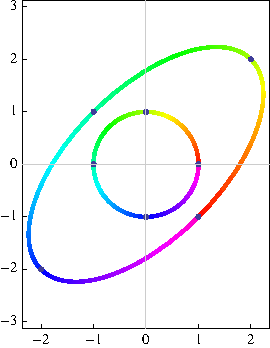
\includegraphics[ width = 2.15in ]{pdf/post_mortemII/2_2_2} &
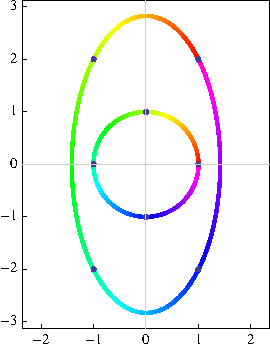
\includegraphics[ width = 2.15in ]{pdf/post_mortemII/2_2_2_t} \\
%%
\ \\
 $\Ap = \frac{1}{4}\mat{rr}{2&-1\\2&1}$ & $\paren{\A{T}}^{+} = \frac{1}{4}\mat{rr}{2&2\\-1&1}$ \\
\ \\
 $\projra = \itwo$ & $\projrat = \itwo$ \\
\ \\
 $\projrap = \mat{cc}{0&0\\0&0}$ & $\projratp = \mat{cc}{0&0\\0&0}$ \\
\ \\
 $\projna = \itwo$ & $\projnat = \itwo$ \\
\ \\
 $\projnap = \mat{cc}{0&0\\0&0}$ & $\projnatp = \mat{cc}{0&0\\0&0}$ \\
\end{tabular}
\end{center}
\label{tab:proj:a}
\caption{The four fundamental projectors for a full rank matrix and its transpose. There is no null space for either $\A{}$ or $\A{T}$.}
\end{table}%

\clearpage
%%
%% 2 x 3
%%
\begin{table}[htdp]
\begin{center}
\begin{tabular}{cc}
  $\A{}x=y$ & $\A{T}y=x$\\
$\mat{ccc}{0&3&0\\1&1&2}\mat{c}{x_{1}\\x_{2}\\x_{3}} = \mat{c}{y_{1}\\y_{2}}$ &
$\mat{cc}{0&1\\3&1\\0&2}\mat{c}{y_{1}\\y_{2}} = \mat{c}{x_{1}\\x_{2}\\x_{3}}$ \\
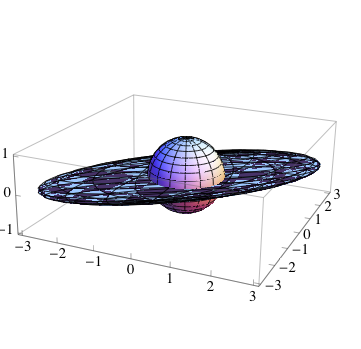
\includegraphics[ width = 2.5in ]{pdf/post_mortemII/3_2_2.png} &
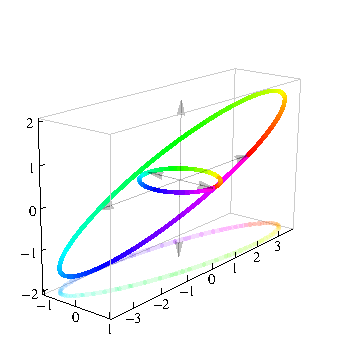
\includegraphics[ width = 2.5in ]{pdf/post_mortemII/3_2_2_t} \\
%%
 $\Ap = \frac{1}{15}\mat{rr}{-2&3\\5&0\\-4&2}$ & $\paren{\A{T}}^{+} = \frac{1}{5}\mat{rrr}{-2&5&-4\\3&0&2}$ \\
\ \\
 $\projra = \itwo$ & $\projrat = \frac{1}{5}\mat{ccc}{1&0&2\\0&1&0\\2&0&4}$ \\
\ \\
 $\projrap = \mat{cc}{0&0\\0&0}$ & $\projratp = \frac{1}{5}\mat{rrr}{4&0&-2\\0&\phantom{-}0&0\\-2&0&1}$ \\
\ \\
 $\projna = \frac{1}{5}\mat{ccc}{1&0&2\\0&1&0\\2&0&4}$ & $\projnat = \itwo$ \\
\ \\
 $\projnap = \frac{1}{5}\mat{rrr}{4&0&-2\\0&\phantom{-}0&0\\-2&0&1}$ & $\projnatp = \mat{cc}{0&0\\0&0}$ \\[15pt]
\end{tabular}
\end{center}
\label{tab:proj:b}
\caption{The four fundamental projectors for a matrix with full row rank. Because the target matrix has full row rank the range spans the domain space and  there is no perpendicular complement.}
\end{table}

\clearpage
%%
%% 3 x 2
%%
\begin{table}[htdp]
\begin{center}
\begin{tabular}{cc}
  $\A{}x=y$ & $\A{T}y=x$\\
$\Aexample \mat{c}{x_{1}\\x_{2}} = \mat{c}{y_{1}\\y_{2}\\y_{3}}$ &
$\Atexample\mat{c}{x_{1}\\x_{2}\\x_{3}} = \mat{c}{y_{1}\\y_{2}}$ \\
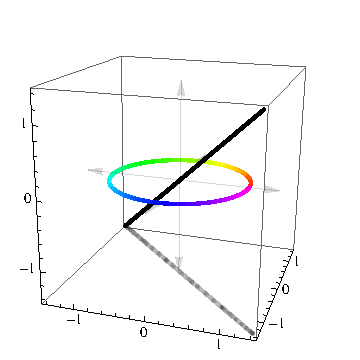
\includegraphics[ width = 2.5in ]{pdf/post_mortemII/3_2_1_a} &
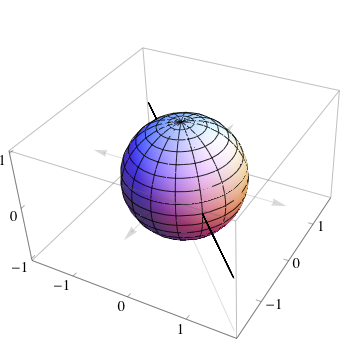
\includegraphics[ width = 2.5in ]{pdf/post_mortemII/3_2_1_t_a} \\
%%
 $\Ap = \Aplus$ & $\paren{\A{T}}^{+} = \frac{1}{6}\Aexample$ \\
\ \\
 $\projra = \frac{1}{3}\Aexample$ & $\projrat = \frac{1}{2}\mat{rr}{1&-1\\-1&1}$ \\
\ \\
 $\projrap = \frac{1}{3}\mat{rrr}{2&1&-1\\1&\phantom{-}2&1\\-1&1&2}$ & $\projratp = \frac{1}{2}\mat{rr}{1&1\\1&1}$ \\
\ \\
 $\projna = \frac{1}{2}\mat{rr}{1&-1\\-1&1}$ & $\projnat = \frac{1}{3}\Aexample$ \\
\ \\
 $\projnap = \frac{1}{2}\mat{rr}{1&1\\1&1}$ & $\projnatp = \frac{1}{3}\mat{rrr}{2&1&-1\\1&\phantom{-}2&1\\-1&1&2}$ \\[10pt]
\end{tabular}
\end{center}
\label{tab:proj:c}
\caption{The four fundamental projectors for a matrix with both row and column rank deficiences. Because the target matrix has full row rank the range spans the domain space and  there is no perpendicular complement.}
\end{table}
\clearpage
\endinput


	
\endinput
\section{Special cases of the pseudoinverse}

Here are some tempting morsels to practice with. This shows the almost symbiotic relationship between the \svdl \ and the generalized matrix inverse. We will be exploiting these three relationships:
\begin{equation}
  \begin{split}
     \A{}  &= \svd{*} = \yrn \essmatrix{} \xtrn{*},\\
     \A{*} &= \svdt{*} = \xrn \essmatrix{T} \ytrn{*},\\
     \Ap   &= \svd{*} = \xrn \essmatrix{-1} \ytrn{*},\\
  \end{split}
\end{equation}
The generic case for the target matrix is $\Amnr$.

%%
\subsection{Underdetermined case}
\label{sec:underdetermined}
Compute the pseudoinverse $\Ap$ when the inverse of the product matrix $\paren{\prdmy{*}}^{-1}$ exists.
Here the target matrix has full row rank and has more columns than row (a wide matrix):
\begin{equation}
  \Accc{m}{n}{m}, \ m\le n.
\end{equation}

Since the inverse of the product matrix $\prdmy{*}$ it must have full rank:
\begin{equation}
  \paren{\prdmy{*}}^{-1} = \paren{\A{*}}^{-1}\paren{\A{}}^{-1}.
\end{equation}
Therefore the target matrix is full rank. Therefore the pseudoinverse matches the standard inverse: 
\begin{equation}
  \Ap = \A{-1}.
\end{equation}

In terms of the SVD, the matrix product reduces to
\begin{equation}
  \begin{split}
    \prdmy{*} & = \paren{\svd{*}}\paren{\svdt{*}}\\
      &= \Y{}\, \sig{}\sig{T}  \Y{*}.
  \end{split}
\end{equation}

Is that your final answer?
\begin{equation}
  \Ap = \A{*}\paren{\prdm{*}}^{-1}
\end{equation}

As an exercise, check that
\begin{equation}
  \A{}\Ap = \Ap\A{} = \I{}.
\end{equation}

%%
\subsection{When $\prdmm{*}=\I{}$}
Because the product matrix
\begin{equation}
  \prdmm{*} = \I{}
\end{equation}
all of the singular values are unity. Therefore
\begin{equation}
  \sig{}=\sig{T}=\I{}.
\end{equation}
\begin{equation}
  \begin{split}
    \prdmm{*}&=\I{},\\
    \paren{\svdt{*}}\paren{\svd{*}}&=\I{},\\
    \X{}\X{*}&=\I{}.
  \end{split}
\end{equation}

	
\endinput
\section{Back to vectors}
Back in section \eqref{sec:vectors} we constructed decompositions for vectors. This leads to speculation about the pseudoinverse for vectors. Does the pseudoinverse exist? What does the pseudoinverse look like? What is the action of the pseudoinverse on the target vector?

Start with the decomposition in \eqref{eq:cases:2vdecomp}:
\begin{equation*}
  \begin{split}
    \svda{T}\\
    \mat{c}{1\\\frac{1}{2}} &= \paren{\frac{1}{\sqrt{5}}\mat{rr}{2&-1\\1&2}}\mat{c}{\frac{\sqrt{5}}{2}\\0}\mat{c}{1}.
  \end{split}
\end{equation*}

The candidate pseudoinverse is this:
\begin{equation}
  \begin{split}
    \mpgia{T}\\
    \mat{cc}{1&\frac{1}{2}} &=\mat{c}{1}\mat{cc}{\frac{\sqrt{5}}{2}&0}\frac{1}{\sqrt{5}}\mat{rr}{2&1\\-1&2}.
  \end{split}
\end{equation}

The actions of this ``inverse'' are the outer and inner products:
\begin{equation}
  \begin{split}
    \rightinv&=v\,v^{\mathrm{T}}=\mat{c}{1\\\frac{1}{2}}\mat{cc}{1&\frac{1}{2}}=\mat{cc}{1&\frac{1}{2}\\\frac{1}{2}&\frac{1}{4}},\\
    \A{+}\A{}&=v^{\mathrm{T}}\,v=\mat{cc}{1&\frac{1}{2}}\mat{c}{1\\\frac{1}{2}} = \frac{5}{4}.
  \end{split}
  \label{eq:mpp:products}
\end{equation}

Do this construction satisfy the Penrose conditions? Start with the first condition:
\begin{equation}
  \begin{split}
    \A{}\paren{\A{+}\A{}}&=\A{}\\
    \mat{c}{1\\\frac{1}{2}}\frac{5}{4}
    &\ne\mat{cc}{1\\\rtwo}\\
  \end{split}
\end{equation}
Clearly then the transpose is not a pseudoinverse due to failure to satisfy all four \index{pseudoinverse!Penrose conditions}Penrose conditions.

We can quickly see from equations \eqref{eq:mpp:products} that the third and fourth conditions are satisfied. However, all four conditions must be satisfied. The vector transpose is \textit{not} a pseudoinverse.




\endinput
\section{The Drazin inverse}
There is another common type of matrix inverse called the Drazin inverse\index{Drazin inverse}. The natural expression for this inverse is in terms of a core-nilpotent matrix decomposition.

Consider a singular matrix $\Ac{m}$ of with an index $k$ defined such that
\begin{equation}
  rank\paren{\A{k}} = \rho
\end{equation}
there exists a nonsingular matrix $\Q{}$ which decomposes the target matrix into a block matrix of the form
\begin{equation}
  \Q{}\A{}\Q{-1} = \mat{c|c}{\pee{}_{\rho\times\rho} & \zero \\[3pt]\hline \zero & \N{}}.
\end{equation}
Here the matrix $\pee{}$ represents the persistent piece and the $\paren{\bys{m-r}}$ block is nilpotent with degree $k$. That is
\begin{equation}
  \N{k} = \zero.
\end{equation}


\endinput

\endinput